\section{すべてをまとめる}

多くの場合、シーケンシャルデータの処理は同じようなパターンで行われます。

\begin{enumerate}
\item  どんな質問をしようとしているのかを把握する。このステップは、問題領域やビジネス領域に位置するため、最も困難な場合が多い。明確な質問があれば、Clojureはあなたが持っているデータを処理して答えを出すためのツールを提供します。それが次の3つのステップです。
\item  データをフィルタリングして、不要な要素を取り除く。
\item 要素を目的の形に変換する。
\item 変換された要素を答えに還元する。
\end{enumerate}


ショッピングカートの例で説明しましょう。オンラインストアでは、カタログ、つまり販売する商品のリストがあります。これらの商品は部門ごとに分けられています。顧客はそれらをカートに入れ、チェックアウトする。このプロセスで、請求記録が作成されます。あなたの顧客は、部門別の売上を要約したレポートを要求しています:すべての決済されたカートについて、部門ごとの総売上はいくらですか?

ドメインモデルは次のとおりです。


\begin{lstlisting}[numbers=none]
(require '[money :refer [make-money +$ *$]])

(defrecord CatalogItem [number dept desc price])
(defrecord Cart        [number customer line-items settled?])
(defrecord LineItem    [quantity catalog-item price])
(defrecord Customer    [cname email membership-number])
\end{lstlisting}

何度もチェックアウトを繰り返すと、カートには\texttt{\#Cart}レコードのベクターが含まれることがあります。


\begin{lstlisting}[numbers=none]
[#Cart{:number 116,
       :customer #Customer{:cname "Danny Tanner",
                           :email "danny@fullhouse.example.com",
                           :membership-number 28374},
       :line-items [
         #LineItem{:quantity 3,
                   :catalog-item #CatalogItem{:number 664,
                                              :dept :clothing,
                                              :desc "polo shirt L",
                                              :amount 2515 :currency :usd},
                   :price #Money{:amount 7545
                                 :currency :usd}
         #LineItem{:quantity 1,
                   :catalog-item #CatalogItem{:number 621,
                                              :dept :clothing,
                                              :desc "khaki pants",
                                              :price #Money{:amount 3500
                                                            :currency
                                                            :usd},
                   :price #Money{:amount 3500
                                 :currency :usd}
                    ],
       :settled? true}, ,,, ]
\end{lstlisting}


これはかなり大きなデータ構造で、次の図のようなクラス図で理解するのが分かりやすいかもしれません。

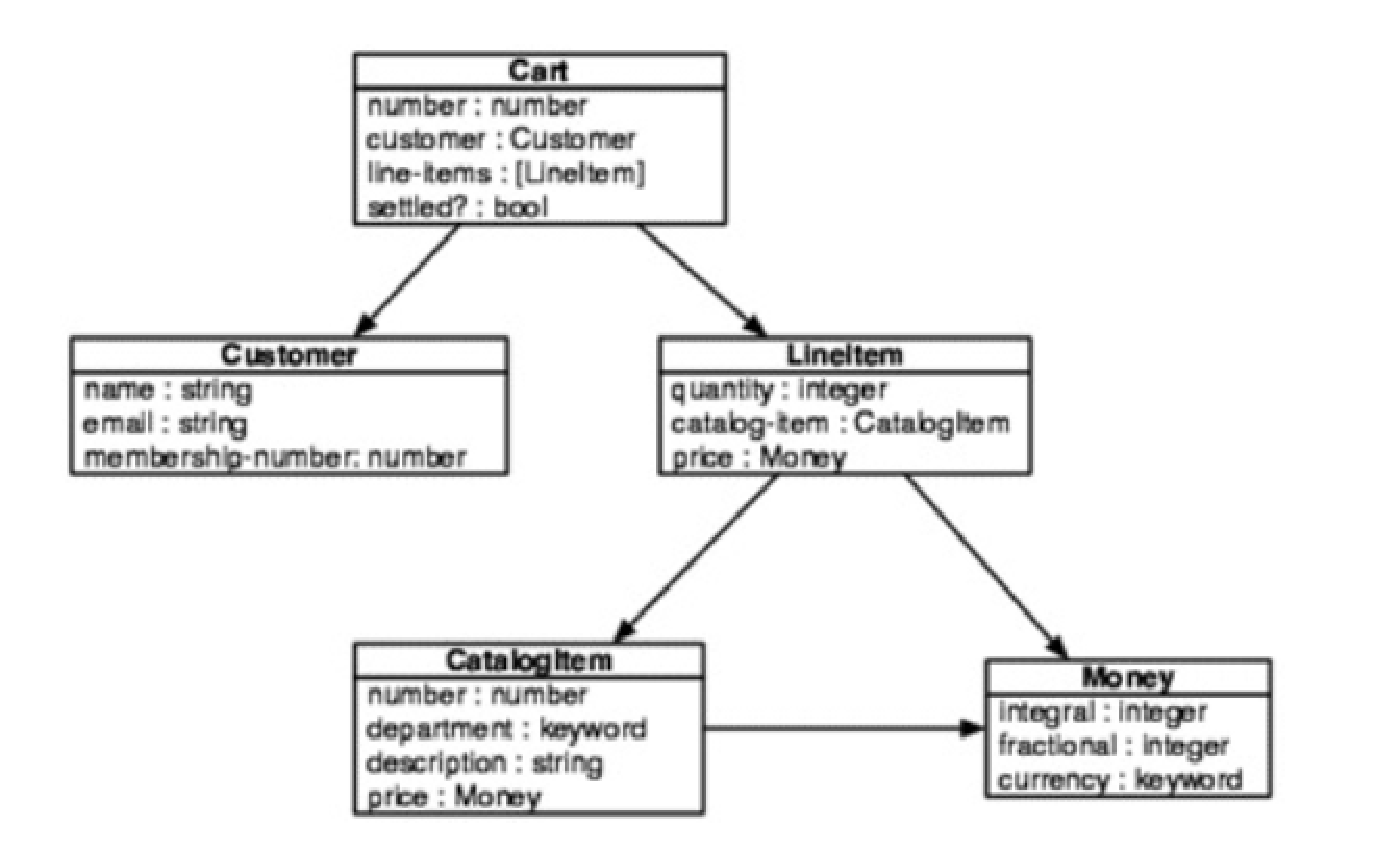
\includegraphics[width=12cm]{fig_03_001.eps}

私たちが求めているのは、もっとシンプルな、部門と金額の対応表です。



\begin{lstlisting}[numbers=none]
{:clothing #Money{:amount 2386424, :currency :usd}
 :toys     #Money{:amount 1163277, :currency :usd}
 ,,, }
\end{lstlisting}

カートの中身から目的の出力まで、順を追って説明しましょう。まず最初にやるべきことは、気になるデータを見つけることです。

\subsection{選択}

シーケンス処理の選択ステップでは、興味のある要素だけを含む部分シーケンスを識別して作成します。カートデータに対してフィルタを使用することで、その要素を取得することができます。

レポートを作成する際、決済されたカートのみを考慮します。決済されるまでは、実際の収益ではなく、潜在的な収益に過ぎないからです。まず、filterを使用してリストのサイズを小さくします。



\begin{lstlisting}[numbers=none]
(defn revenue-by-department [carts]
  (->> (filter :settled? carts)
       ,,,))
\end{lstlisting}

キーワード \texttt{:settled?} を関数として使用すると、 \texttt{:settled?} が\texttt{true}でないカートをすべてフィルタリングすることができます。

\subsection{トランスフォーメーション}

これで一連の決済カートが揃ったので、部門別に収益を分離することができるようになりました。カートは一切必要なく、品目とカタログ品だけが必要なことがわかります。今は一歩ずつ進めていきましょう。次のステップは、すべてのラインアイテムのシーケンスを作成することです。


\begin{lstlisting}[numbers=none]
(defn revenue-by-department [carts]
  (->> (filter :settled? carts)
       (mapcat :line-items)
       ,,,))
\end{lstlisting}

\texttt{(mapcat :line-items ,,)} の結果は、このようになります。


\begin{lstlisting}[numbers=none]
[#LineItem{:quantity 3,
           :catalog-item #CatalogItem{:number   664,
                                      :dept  :clothing,
                                      :desc "polo shirt L",
                                      :price #Money{:amount 2515
                                                    :currency :usd}},
           :price #Money{:amount   7545
                         :currency :usd}},
 #LineItem{:quantity 1,
           :catalog-item #CatalogItem{:number 621,
                                      :dept :clothing,
                                      :desc "khaki pants",
                                      :price #Money{:amount 3500
                                                    :currency :usd}},
           :price #Money{:amount   3500
                         :currency :usd}}, ,,, ]
\end{lstlisting}

\texttt{mapcat}関数は、行項目ベクターの内容を集積したものを構築する。

\begin{itembox}[l]{mapcatとmap + flattenの使い分け}
\texttt{mapcat}の代わりに、\texttt{map}と\texttt{flatten}を併用することで、同様の結果を得ることができます。\texttt{flatten}を使いたくなったら、一歩戻って、そもそも\texttt{flatten}する必要がある構造を作らないようにしましょう。最も一般的なのは、\texttt{map}ではなく\texttt{mapcat}を使うことです(\texttt{map}と\texttt{concatenate}を行うため)。
\end{itembox}

次のステップは、各ラインアイテムから、カタログアイテムの :dept 値とラインアイテムの親の :price 値という気になるデータのマップを抽出することである。これは map と line-summary ヘルパー関数によって行われます。
